\documentclass[11pt,a4paper]{article}
\usepackage[spanish,es-tabla]{babel}
\usepackage[utf8]{inputenc}
\usepackage[T1]{fontenc}
\usepackage{geometry}
\usepackage{graphicx}
\usepackage{booktabs}
\usepackage{longtable}
\usepackage{array}
\usepackage{enumitem}
\usepackage{xcolor}
\usepackage{hyperref}
\geometry{margin=2.5cm}
\graphicspath{{figures/}{../stress/2026-07-05_local-smoke_v1/}}
\hypersetup{colorlinks=true, linkcolor=blue, urlcolor=blue}

\title{Servidor Proxy SOCKS5 con Protocolo de Monitoreo}
\author{Grupo: \textit{completar integrantes}}
\date{Protocolos de Comunicación -- 2026C1}

\begin{document}
\maketitle

\begin{abstract}
Se desarrolló un servidor proxy SOCKS5 en C11 con I/O no bloqueante multiplexado,
autenticación usuario/contraseña, conexión TCP saliente a IPv4, IPv6 y FQDN,
resolución DNS fuera del hilo del selector, métricas volátiles, registro de
accesos y un protocolo propio de monitoreo/configuración con cliente CLI. El
alcance cubre la primera entrega; el monitoreo de credenciales POP3 queda fuera.
\end{abstract}

\tableofcontents
\clearpage

\section{Descripción de protocolos y aplicaciones}

La aplicación servidor actúa como intermediario entre clientes SOCKS5 y
servicios TCP. En el mismo proceso ofrece un plano de administración separado,
al que accede la aplicación cliente de terminal. Esta división evita que las
operaciones administrativas se confundan con el tráfico que retransmite el
proxy.

\subsection{SOCKS5}

El proxy acepta autenticación usuario/contraseña y el comando \texttt{CONNECT}
para destinos IPv4, IPv6 o FQDN. Después de establecer la conexión saliente,
retransmite bytes en ambos sentidos sin interpretar el protocolo de aplicación.
Si un nombre resuelve a varias direcciones, conserva la lista y prueba la
siguiente cuando una conexión falla. La decisión importante no fue reproducir
los pasos de RFC1928 y RFC1929, sino integrarlos con lecturas parciales y con una
máquina de estados que nunca presupone cómo se segmentan los datos en TCP.

\subsection{Protocolo de monitoreo}

El Protocolo de Monitoreo y Configuración (PMC) usa una conexión TCP persistente.
Es textual y orientado a líneas terminadas en \texttt{CRLF}. Cada pedido empieza
con un nombre de comando hasta el primer espacio o fin de línea; los campos
restantes se separan por un único espacio. Para cada pedido el servidor devuelve
una respuesta que comienza con \texttt{+OK} o \texttt{-ERR}. Antes de operar, el
cliente negocia la versión y autentica una credencial administrativa.

Los comandos implementados son \texttt{ADD-USER}, \texttt{DEL-USER},
\texttt{LIST-USERS}, \texttt{METRICS}, \texttt{GET-CONFIG},
\texttt{SET-CONFIG} y \texttt{QUIT}. Las respuestas multi-línea usan prefijo de
cantidad para delimitar la respuesta sin depender del cierre de la conexión. La
gramática, los estados y cada respuesta posible se especifican en
\texttt{docs/mgmt-protocol-rfc.md}.

El cliente de terminal oculta la negociación y el formato de cable. Traduce
subcomandos como \texttt{metrics} o \texttt{add-user} a pedidos PMC y presenta
resultados etiquetados, listas y mensajes de error, en lugar de copiar las líneas
recibidas del socket.

\section{Problemas encontrados}

\begin{longtable}{p{0.25\linewidth}p{0.65\linewidth}}
\toprule
\textbf{Problema} & \textbf{Resolución} \\
\midrule
Portabilidad Linux/macOS & Se usaron macros de plataforma en el Makefile para
exponer APIs POSIX bajo C11 sin romper macOS. \\
I/O parcial y pipelining & Los parsers consumen desde buffers y preservan bytes
sobrantes para el siguiente estado. Esto evita perder AUTH o REQUEST enviados en
el mismo segmento. \\
Errores del selector base & Se corrigieron casos de flags no bloqueantes,
límites de fd y headers no autocontenidos. \\
DNS bloqueante & La resolución se aisló en hilos \texttt{pthread} dedicados a
\texttt{getaddrinfo}; el resultado vuelve al selector por notificación. \\
Reuso de fd durante DNS & Las notificaciones de DNS llevan identidad del objeto
de conexión para no despachar un resultado viejo sobre una conexión nueva. \\
Half-close pre-COPY & Si el cliente envía payload temprano y hace half-close
mientras el \texttt{connect} está pendiente, el proxy conserva el payload y lo
drena al origin al entrar en \texttt{COPY}. \\
\bottomrule
\end{longtable}

\section{Limitaciones de la aplicación}

El selector actual usa \texttt{pselect} y queda limitado por \texttt{FD\_SETSIZE}.
Una conexión SOCKS5 establecida consume dos file descriptors principales:
cliente-proxy y proxy-origen. Por eso el techo real debe medirse en el entorno
de entrega, no inferirse sólo desde el código.

Las métricas se conservan sólo mientras vive el proceso. El access-log se escribe
de forma síncrona con \texttt{fprintf}/\texttt{fflush}; esto facilita inspeccionar
cada registro, pero puede introducir latencia cuando el dispositivo de salida es
lento.

El apagado controlado tiene una decisión explícita: una segunda señal corta el
drenaje graceful de conexiones activas, pero no destruye el selector ni el pool
mientras haya resoluciones DNS pendientes. Esto evita use-after-free, al costo de
esperar si \texttt{getaddrinfo} tarda.

El PMC autentica al administrador pero no cifra el canal. Debe utilizarse dentro
de una red administrativa controlada o acompañado por una capa de transporte
segura.

\section{Posibles extensiones}

\begin{itemize}[nosep]
  \item migrar el selector a \texttt{poll}, \texttt{epoll} o \texttt{kqueue} para
  superar \texttt{FD\_SETSIZE};
  \item persistir métricas y rotar logs;
  \item agregar TLS o un esquema de autenticación más fuerte al PMC;
  \item exponer timeouts y más parámetros de configuración en runtime;
  \item exportar métricas en un formato apto para monitoreo externo.
\end{itemize}

\section{Conclusiones}

El principal aprendizaje fue que I/O no bloqueante no significa reemplazar una
llamada bloqueante por otra con una bandera. Cada evento habilita sólo una parte
del trabajo: una lectura puede traer medio mensaje, una escritura puede aceptar
algunos bytes y un \texttt{connect} puede quedar pendiente. Modelar ese progreso
en estados y buffers hizo posible conservar datos y aplicar contrapresión sin
detener a las demás conexiones.

La resolución de nombres mostró otro aspecto menos evidente: sacar
\texttt{getaddrinfo} del hilo principal resuelve el bloqueo, pero introduce un
problema de identidad y tiempo de vida. Tuvimos que razonar qué ocurre si el
cliente se desconecta, el descriptor se reutiliza o el proceso comienza a
apagarse mientras la resolución continúa. Aprendimos que la concurrencia debe
analizarse por propiedad de los datos y no sólo por la cantidad de hilos.

Diseñar PMC también cambió nuestra forma de describir un protocolo. Los ejemplos
sirven para ilustrar, pero no reemplazan una gramática, una máquina de estados ni
reglas que delimiten cada respuesta. El prefijo de cantidad en respuestas
multilínea y el orden en pipelining surgieron de preguntarnos cómo podría un
cliente independiente interpretar el flujo sin conocer nuestra implementación.

Por último, las mediciones de carga nos enseñaron a separar una observación de
una afirmación de capacidad. Las gráficas permiten comparar throughput, latencia
y errores bajo las combinaciones ejecutadas; no demuestran por sí solas un máximo
universal. El límite de \texttt{pselect}, dado por \texttt{FD\_SETSIZE}, y el consumo de dos
descriptores por conexión explican por qué el entorno y la metodología forman
parte del resultado.

\section{Ejemplos de prueba}

\begin{longtable}{>{\raggedright\arraybackslash}p{0.32\linewidth}>{\raggedright\arraybackslash}p{0.22\linewidth}>{\raggedright\arraybackslash}p{0.36\linewidth}}
\toprule
\textbf{Comando} & \textbf{Estado} & \textbf{Observación} \\
\midrule
\texttt{make clean \&\& make} & Verificado local y Pampero & Compila
\texttt{bin/server} y \texttt{bin/client} sin warnings visibles. \\
\texttt{make test} & Verificado local y Pampero & Unitarios C del parser,
usuarios, métricas, logger, selector bloqueante y relay. \\
\texttt{make check PORT=12080} & Verificado local y Pampero & Flujos completos
de negociación, autenticación, conexión, relay, DNS, métricas y PMC. \\
\texttt{make valgrind PORT=...} & Verificado en Pampero & Valgrind con tráfico:
0 errores, 0 leaks definitivos/indirectos/posibles. \\
\texttt{strace} sobre relay HTTP & Verificado en Pampero & En ambos sentidos se
observó \texttt{recvfrom} $\rightarrow$ \texttt{sendto} sin un
\texttt{pselect6} intermedio. \\
\texttt{test/stress/run\_stress.py} & Corrida local acotada & Genera CSV y
figuras reproducibles para las combinaciones elegidas. \\
\bottomrule
\end{longtable}

\subsection{Corrida Pampero/Linux}

La corrida remota se ejecutó en \texttt{pampero.it.itba.edu.ar}, Linux
\texttt{7.0.9-arch1-1}, GCC \texttt{16.1.1 20260625}. El build
\texttt{make clean \&\& make} terminó con \texttt{BUILD OK}.

Los unitarios reportaron todos los casos OK y cubrieron:
\begin{itemize}[nosep]
  \item negociación, autenticación y parseo de pedidos fragmentados;
  \item conexión, relay bidireccional, cierres parciales y contrapresión;
  \item notificaciones del selector, métricas y registro de accesos.
\end{itemize}

Las integraciones terminaron sin fallas y ejercitaron los mismos comportamientos
sobre sockets reales. El único caso no ejecutado requería que el entorno
resolviera un dominio a varias direcciones para forzar el reintento; esa
precondición no estaba disponible en la corrida.

Valgrind con tráfico real reportó:
\begin{itemize}[nosep]
  \item \texttt{FILE DESCRIPTORS: 2 open (2 inherited) at exit};
  \item \texttt{definitely lost: 0 bytes}, \texttt{indirectly lost: 0 bytes} y
  \texttt{possibly lost: 0 bytes};
  \item \texttt{ERROR SUMMARY: 0 errors from 0 contexts}.
\end{itemize}
Los \texttt{5,658 bytes} \texttt{still reachable} se consideran alcanzables del
entorno/libc, no leaks definitivos del programa.

\subsection{Stress local}

El banco de stress se genera con \texttt{test/stress/run\_stress.py}. El script
levanta un origin controlado, ejecuta el servidor SOCKS5, consulta métricas por
PMC y escribe CSV bajo un directorio de salida. Los parámetros principales son:

\begin{itemize}[nosep]
  \item concurrencia: cantidad de conexiones simultáneas por caso;
  \item payload: bytes transferidos por conexión;
  \item modo de destino: \texttt{ipv4} o \texttt{fqdn};
  \item métricas recolectadas: conexiones OK/fallidas, bytes, wall time,
  throughput, tasa de conexiones, latencias p50/p95, REP no exitosos y deltas
  de métricas PMC.
\end{itemize}

La evidencia versionada corresponde a una corrida local acotada en macOS,
guardada en:
\begin{center}
\texttt{docs/stress/2026-07-05\_local-smoke\_v1/}
\end{center}

La corrida usó concurrencias 5 y 20, payloads 1024 y 8192 bytes, destinos IPv4 y
FQDN, y una repetición por combinación. También hubo una prueba local adicional de
500 conexiones con \texttt{conn\_ok=500} y \texttt{conn\_failed=0}. No se
presenta como máximo absoluto del servidor ni como barrido completo en Pampero.

\IfFileExists{../stress/2026-07-05_local-smoke_v1/2026-07-05_fig-throughput-vs-concurrency_v1.png}{
\begin{figure}[htbp]
  \centering
  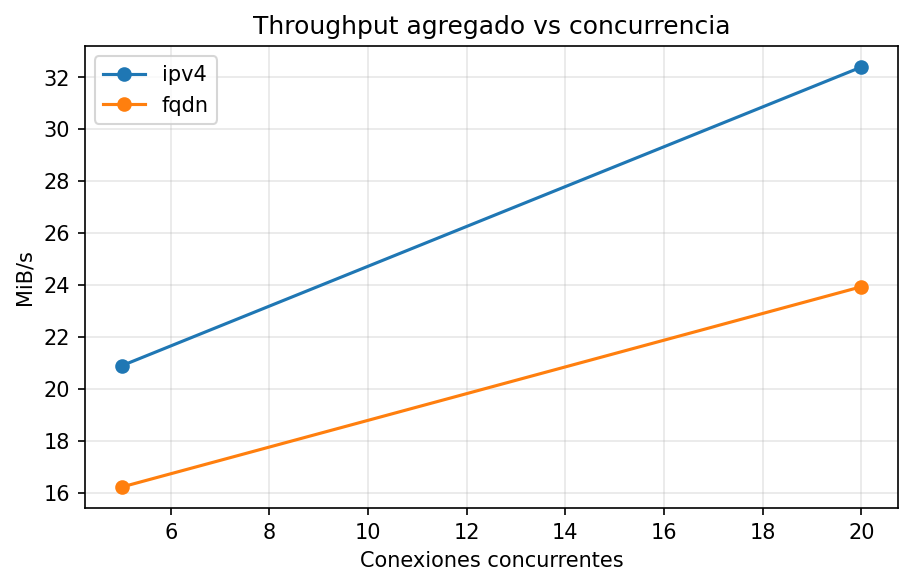
\includegraphics[width=0.82\linewidth]{2026-07-05_fig-throughput-vs-concurrency_v1.png}
  \caption{Throughput agregado de la corrida local por concurrencia y modo de destino.}
\end{figure}
}{}

\IfFileExists{../stress/2026-07-05_local-smoke_v1/2026-07-05_fig-error-rate-vs-concurrency_v1.png}{
\begin{figure}[htbp]
  \centering
  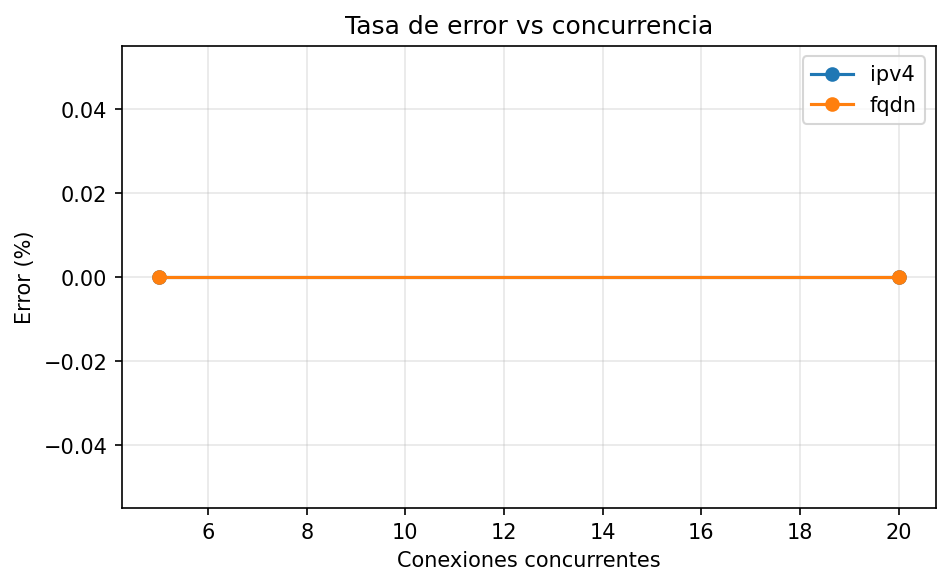
\includegraphics[width=0.82\linewidth]{2026-07-05_fig-error-rate-vs-concurrency_v1.png}
  \caption{Tasa de error de la corrida local. No hubo conexiones fallidas.}
\end{figure}
}{}

\IfFileExists{../stress/2026-07-05_local-smoke_v1/2026-07-05_fig-latency-p50-p95-vs-concurrency_v1.png}{
\begin{figure}[htbp]
  \centering
  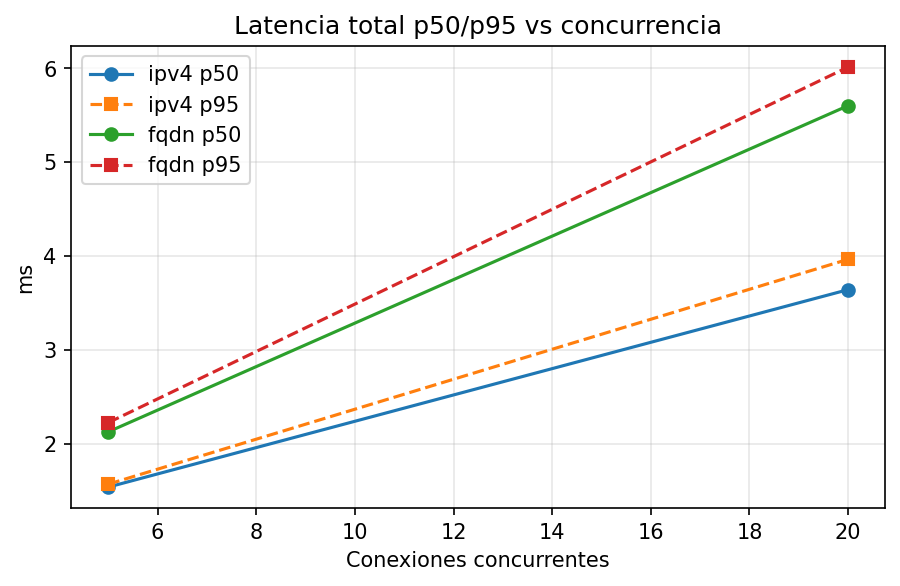
\includegraphics[width=0.82\linewidth]{2026-07-05_fig-latency-p50-p95-vs-concurrency_v1.png}
  \caption{Latencias p50/p95 totales de la corrida local.}
\end{figure}
}{}

\section{Guía de instalación}

Dependencias:
\begin{itemize}[nosep]
  \item compilador C11 (\texttt{gcc} o \texttt{clang});
  \item \texttt{make};
  \item \texttt{python3} para integraciones y stress;
  \item \texttt{valgrind} en Linux/Pampero para memoria/fds;
  \item \texttt{matplotlib} si se quieren regenerar gráficos de stress;
  \item \texttt{rsync} y \texttt{ssh} para el runner de Pampero.
\end{itemize}

Compilación:
\begin{verbatim}
make clean && make
\end{verbatim}

Artefactos generados:
\begin{itemize}[nosep]
  \item \texttt{bin/server}: servidor SOCKS5 + PMC;
  \item \texttt{bin/client}: cliente CLI del PMC;
  \item \texttt{docs/report/main.pdf}: este informe.
\end{itemize}

Verificación remota recomendada:
\begin{verbatim}
PAMPERO_USER=<usuario> bash scripts/run-on-pampero.sh 12080
\end{verbatim}

El script sube el repo a Pampero, recompila desde cero y ejecuta unitarios,
integraciones sobre sockets y Valgrind con tráfico real.

\section{Instrucciones para la configuración}

Opciones principales del servidor:
\begin{verbatim}
./bin/server [OPCIONES]
  -l <addr>        direccion SOCKS, default 0.0.0.0
  -p <port>        puerto SOCKS, default 1080
  -L <addr>        direccion PMC, default 127.0.0.1
  -P <port>        puerto PMC, default 8080
  -u <name>:<pass> usuario SOCKS5
  --admin u:p      credencial de administracion PMC
  -N               desactiva disectores
  -h / -v          ayuda / version
\end{verbatim}

El tamaño de buffer se puede consultar y cambiar para conexiones nuevas mediante
el PMC con \texttt{GET-CONFIG buffer-size} y \texttt{SET-CONFIG buffer-size N}.

\section{Ejemplos de configuración y monitoreo}

Ejemplos con el cliente:
\begin{verbatim}
./bin/client --admin admin:s3cr3t metrics
./bin/client --admin admin:s3cr3t add-user pablito pass1234
./bin/client --admin admin:s3cr3t list-users
./bin/client --admin admin:s3cr3t get-config buffer-size
./bin/client --admin admin:s3cr3t set-config buffer-size 32768
./bin/client --admin admin:s3cr3t del-user pablito
\end{verbatim}

Ejemplo de sesión cruda PMC:
\begin{verbatim}
C: HELLO 1
S: +OK 1
C: AUTH admin s3cr3t
S: +OK
C: METRICS
S: +OK 5
S: historic-connections 10
S: concurrent-connections 0
S: bytes-transferred 123456
S: configured-users 2
S: failed-connections 1
\end{verbatim}

\section{Documento de diseño del proyecto}

El servidor usa tres piezas centrales del toolkit: \texttt{selector},
\texttt{stm} y \texttt{buffer}. El selector concentra los eventos de sockets; la
máquina de estados separa cada fase del protocolo; los buffers resuelven
lecturas y escrituras parciales.

\subsection{Estados SOCKS5}

\begin{center}
\texttt{HELLO -> AUTH -> REQUEST -> RESOLV? -> CONNECTING -> REQUEST\_WRITE -> COPY -> DONE}
\end{center}

\texttt{COPY} mantiene dos direcciones de relay: cliente a origen y origen a
cliente. Cada dirección tiene su estado de lectura/escritura; al recibir EOF en
un sentido se drena lo pendiente y se propaga \texttt{shutdown(SHUT\_WR)} al par.
Cuando una lectura produce datos, el relay realiza inmediatamente un único
intento de escritura no bloqueante sobre el socket opuesto. En el caso favorable
esto evita una vuelta adicional \texttt{pselect} $\rightarrow$ \texttt{write}; ante una escritura
parcial o \texttt{EAGAIN}, conserva los bytes pendientes en el buffer y delega el
drenaje posterior al selector. El límite de un intento por activación preserva la
equidad del event loop entre conexiones concurrentes.

\subsection{DNS y lifetime}

La resolución FQDN corre en un hilo detached que sólo ejecuta \texttt{getaddrinfo}
y notifica al selector. La notificación lleva identidad del objeto de conexión y
cleanup asociado. El proceso de apagado espera a que no haya resoluciones DNS en
vuelo antes de destruir selector y pool.

\subsection{PMC}

El PMC tiene su propio listener y su propia STM, pero comparte el mismo selector
del servidor. El cliente CLI usa I/O bloqueante por simplicidad, permitido por la
consigna, y encapsula el framing del protocolo.


\end{document}
